\section{Specifikation og Analyse}

I følgende afsnit vil der være beskrevet de overvejelser der har været lavet, i forbindelse med det overordnede design af systemet.

\begin{figure}[H]
	\centering
	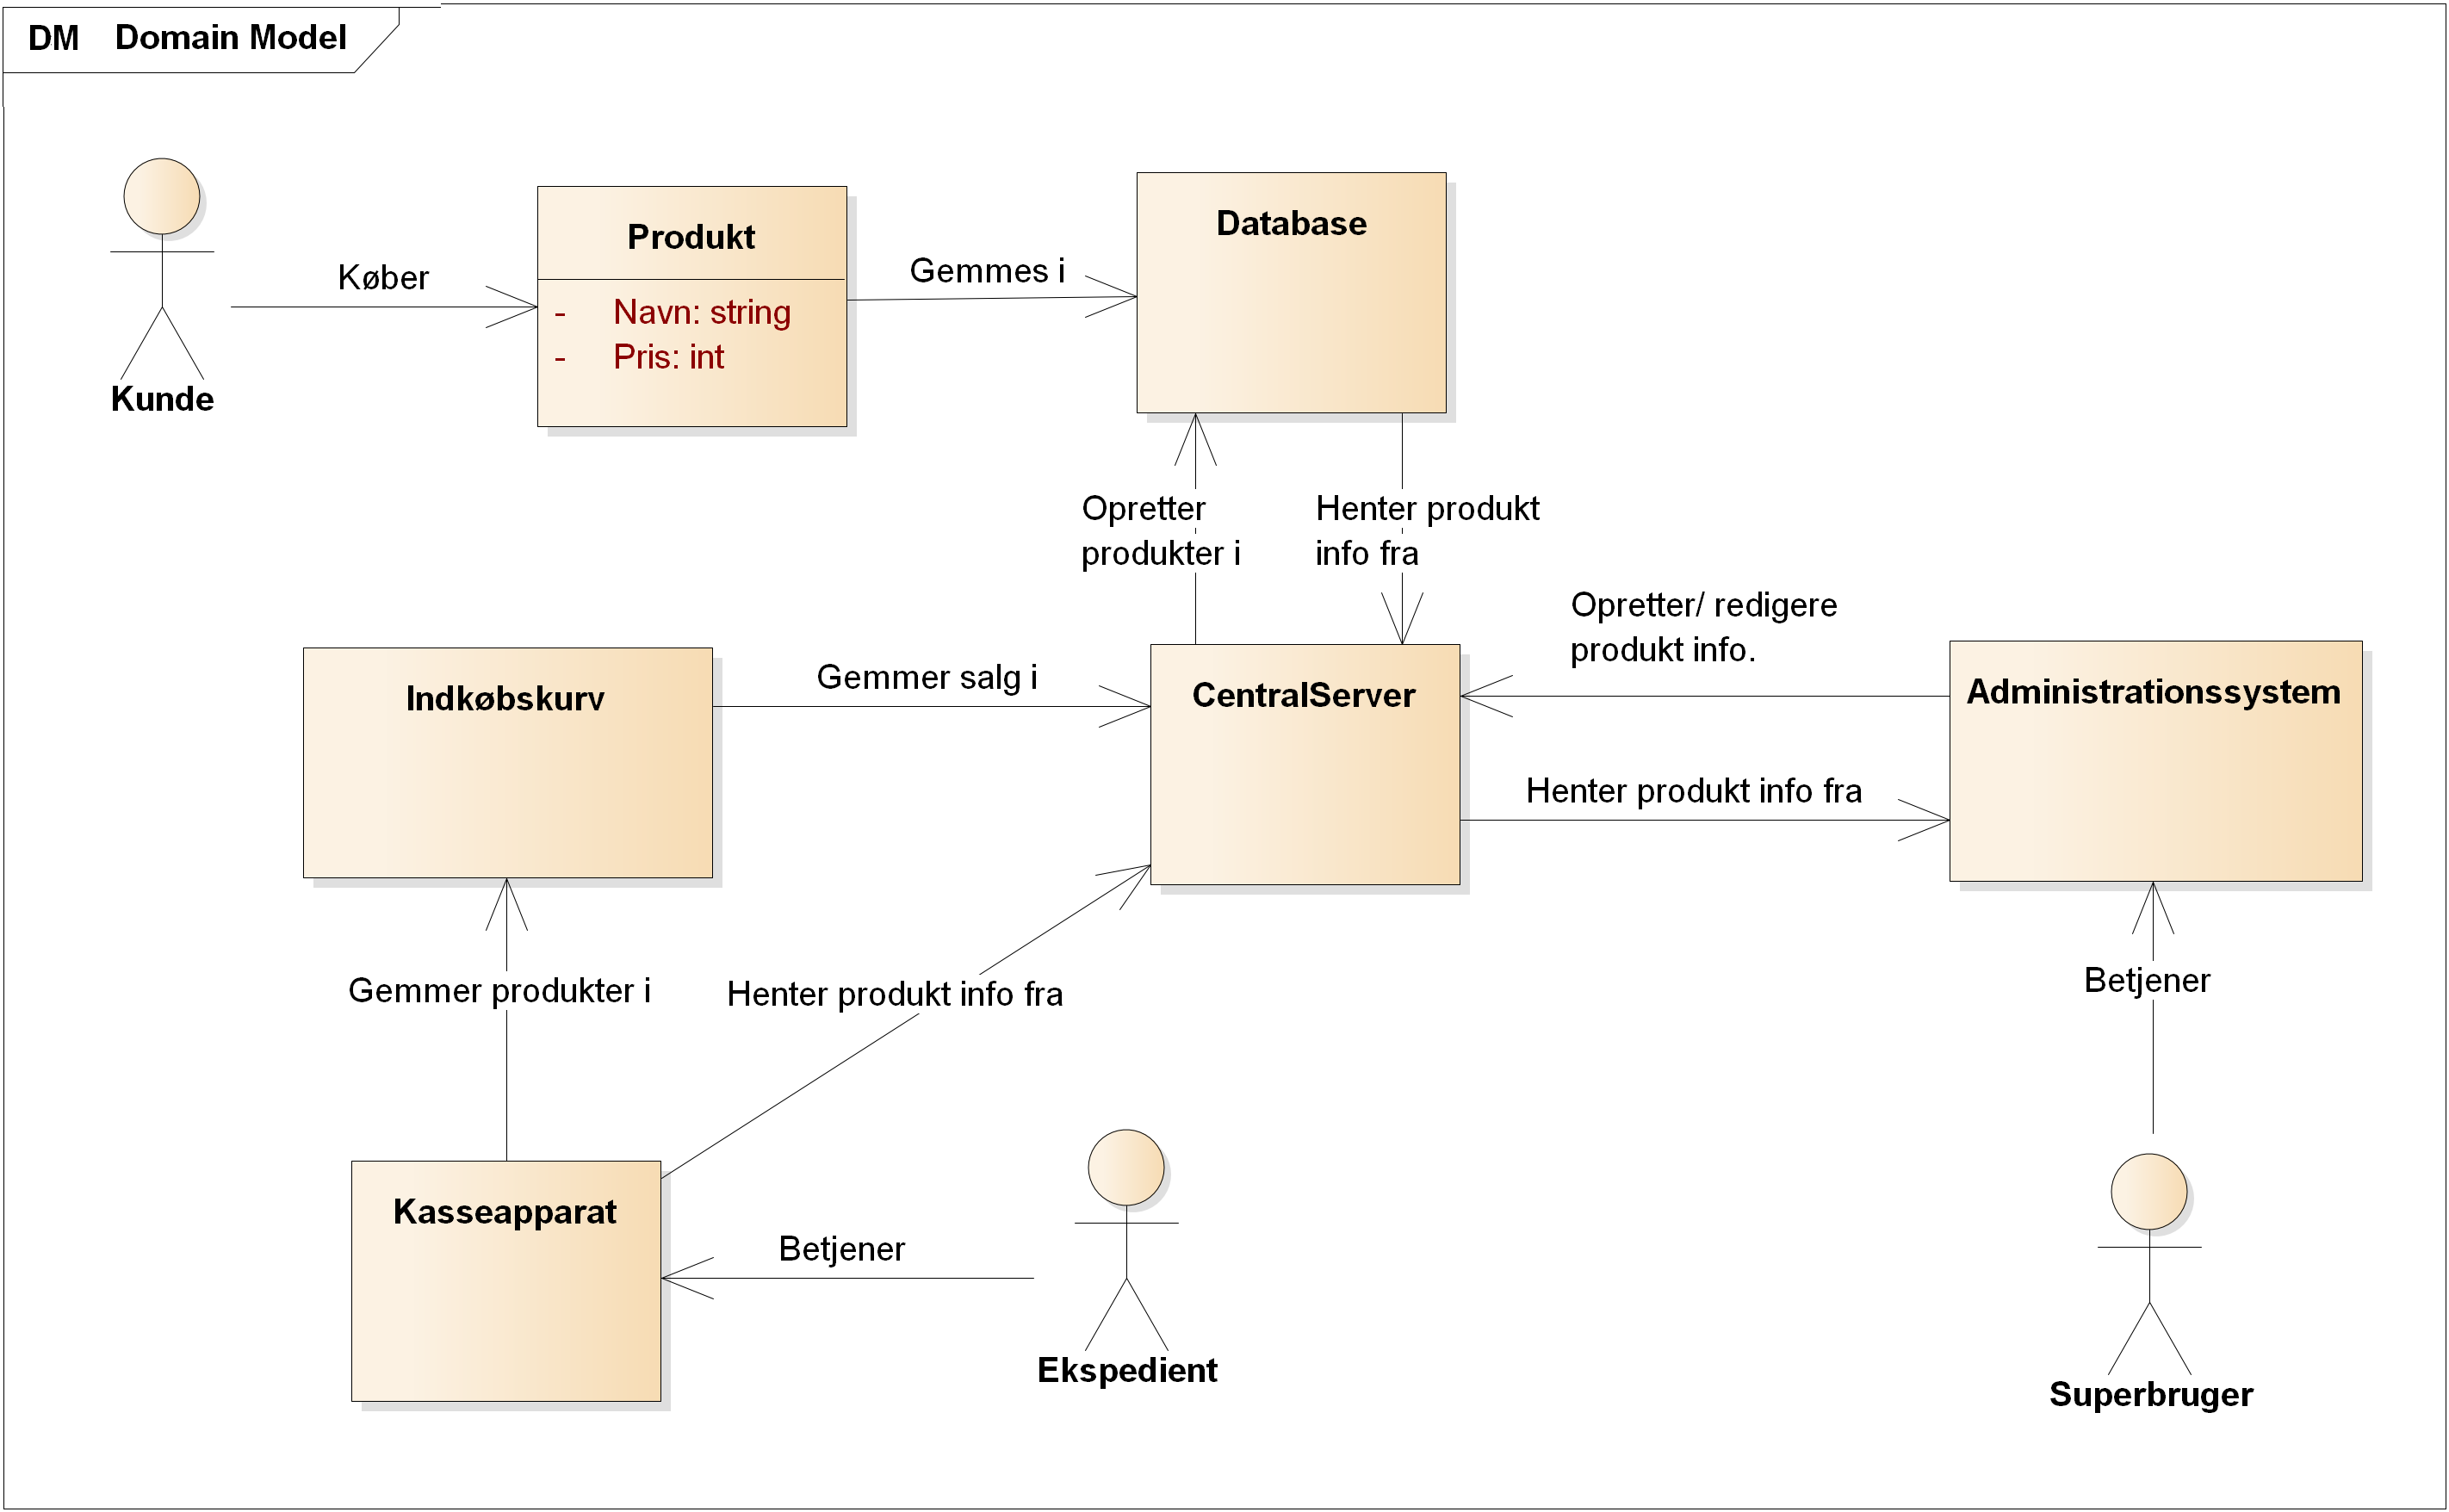
\includegraphics[width=1\textwidth]{Projektbeskrivelse/Images/DomainModel.png}
	\caption{Domænemodel for salgssystemet}
	\label{fig:domain}
\end{figure}


\textbf{Overodnet struktur}\\
Den overordnede struktur er blevet lavet som 3 delsystemer og et delt bibliotek. Årsagen til dette ligger i at kunne afkoblet de forskellige dele som ikke havde noget med hinanden at gøre. Eksempelvis bør et kasseapperat ikke kende til et administrationssystem og vica verca.\\
Derfor blev det besluttet at samle dataen i en central server, deraf navnet CentralServer. På den måde kan de interesserede systemer skrive og læse fra CentralServer, uden at skulle kende til hinanden.\\
I den forbindelse er det vigtigt at være enige om den data der udveksles. Derfor blev det besluttet at lave et delt bibliotek som standardiserer de brugte datamodeller. Det tillader at hvis en eventuel ændring skulle foretages i en datamodel, var det til dels kun nødvendigt at ændre i det delte bibliotek.\\
\\

\textbf{Kommunikation}\\
Til at kommunikkere med CentralServer og modsatrettet, blev det besluttet at benytte TCP/IP~\cite{tcpip} som protokol. Dette giver følgende fordele:

\begin{itemize}
	\item TCP garanterer fejlfri overførsel
	\item TCP er fuld duplex. 
	\item Serveren kan stå hvor som helst i verdenen.
	\item Nemt at udvikle til.
\end{itemize}

